\documentclass{article}
\usepackage[utf8]{inputenc}
% are all of these packages really necessary?
% no.
% i'm just too lazy to only grab the packages i want for a specific
% document, so i just glob all of my most commonly used packages together
% this is bad practice.
\usepackage{amsmath,amsthm,amssymb,amsfonts, fancyhdr, color, comment, graphicx, environ, mdframed, soul, calc, enumitem, mdframed, xcolor, geometry, empheq, mathtools, tikz, pgfplots, caption, subcaption, hyperref}

\usetikzlibrary{external}
\tikzexternalize[prefix=tikz/,optimize command away=\includepdf]

%tikzpicture
\usepackage{tikz}
\usepackage{scalerel}
\usepackage{pict2e}
\usepackage{tkz-euclide}
\usetikzlibrary{calc}
\usetikzlibrary{patterns,arrows.meta}
\usetikzlibrary{shadows}
\usetikzlibrary{external}

%pgfplots
\usepackage{pgfplots}
\pgfplotsset{compat=newest}
\usepgfplotslibrary{statistics}
\usepgfplotslibrary{fillbetween}
\usepgfplotslibrary{polar}

\tikzset{external/export=true}
\pgfplotsset{
    standard/.style={
    axis line style = thick,
    trig format=rad,
    enlargelimits,
    axis x line=middle,
    axis y line=middle,
    enlarge x limits=0.15,
    enlarge y limits=0.15,
    every axis x label/.style={at={(current axis.right of origin)},anchor=north west},
    every axis y label/.style={at={(current axis.above origin)},anchor=south east}
    }
}
\newcommand*\widefbox[1]{\fbox{\hspace{2em}#1\hspace{2em}}}
% Command "alignedbox{}{}" for a box within an align environment
% Source: http://www.latex-community.org/forum/viewtopic.php?f=46&t=8144
\newlength\dlf  % Define a new measure, dlf
\newcommand\alignedbox[2]{
% Argument #1 = before & if there were no box (lhs)
% Argument #2 = after & if there were no box (rhs)
&  % Alignment sign of the line
{
\settowidth\dlf{$\displaystyle #1$}  
    % The width of \dlf is the width of the lhs, with a displaystyle font
\addtolength\dlf{\fboxsep+\fboxrule}  
    % Add to it the distance to the box, and the width of the line of the box
\hspace{-\dlf}  
    % Move everything dlf units to the left, so that & #1 #2 is aligned under #1 & #2
\boxed{#1 #2}
    % Put a box around lhs and rhs
}
}

\renewcommand{\arraystretch}{1.5}

\hypersetup{
    colorlinks=true,
    linkcolor=blue,
    filecolor=magenta,      
    urlcolor=cyan,
    pdftitle={Homework 7 Solutions},
    pdfpagemode=UseOutlines,
    bookmarksopen=true,
    pdfauthor={Christina Phan}
}
\newcommand{\lrp}[1]{\left( #1 \right)}
\newcommand{\abs}[1]{\left\vert #1 \right\vert}
\newcommand{\lra}[1]{\left\langle #1 \right\rangle}
\newcommand{\lrb}[1]{\left[ #1 \right]}
\newcommand{\iintR}[0]{\iint\limits_{R}}

\geometry{letterpaper, portrait, margin=1in}
\renewcommand{\footrulewidth}{0.8pt}
\setlength\parindent{0pt}
\pagestyle{fancy}
\lhead{Christina Phan}
\rhead{MAT 21D} 
\chead{\textbf{Homework 7 Solutions}}

\newcommand{\Solution}{\textit{Solution}}
\pgfplotsset{compat=1.18}
\begin{document}
\phantomsection
\addcontentsline{toc}{section}{Problem 1}\textbf{Problem 1}

Use $u=x-y$, $v=2x+y$ to evaluate the integral $\displaystyle \iint_R 2x^2-xy-y^2\,dA$ over the region $R$ bounded by the lines $y=4-2x$, $y=7-2x$, $y=x-2$, and $y=x+1$.

\Solution

\phantomsection
\addcontentsline{toc}{subsection}{Finding u, v, partials, and Jacobian}\textbf{Finding $u$, $v$, partials, and Jacobian}

First, let's find $x$ and $y$ in terms of $u$ and $v$. To do that, let's \textit{add} $u$ and $v$ together to get rid of the $y$'s. Then, we can solve for $y$ in the $u$ or $v$ equation and plug in what we know about $x$.

Here, we \textit{add} $u$ and $v$ because we want to get rid of $y$. If we subtracted $u$ and $v$, $y$ would still be there, so it'll be useless.
\begin{align*}
    u+v&=(x-y)+(2x+y)=3x\\
    \implies x &= \frac{1}{3}u+\frac{1}{3}v\\
    y &= v - 2x = v - 2\lrp{\frac{1}{3}u+\frac{1}{3}v}=-\frac{2}{3}u+\frac{1}{3}v\tag{let's use $v=2x+y$ and solve for $y$}
\end{align*}
Now, let's get our partials and Jacobian.
\begin{align*}
     \frac{\partial x}{\partial u} &= \frac{1}{3}\\
    \frac{\partial x}{\partial v} &=\frac{1}{3}\\
    \frac{\partial y}{\partial u}&= -\frac{2}{3}\\
     \frac{\partial y}{\partial v}&= \frac{1}{3}\\
    \begin{vmatrix}
    \frac{\partial x}{\partial u} & \frac{\partial x}{\partial v}\\
    \frac{\partial y}{\partial u} & 
    \frac{\partial y}{\partial v}
    \end{vmatrix}&=\begin{vmatrix}
      \frac{1}{3} & \frac{1}{3}\\
      -\frac{2}{3} & \frac{1}{3}
    \end{vmatrix}=\lrp{\frac{1}{3}\times\frac{1}{3}}-\lrp{\frac{1}{3}\times\lrp{-\frac{2}{3}}}=\frac{1}{3}
\end{align*}
\phantomsection
\addcontentsline{toc}{subsection}{Getting the uv region}\textbf{Getting the $uv$ region}

Let's translate our $xy$ region into a $uv$ region.

For $y=4-2x$,
\begin{align*}
    y&=4-2x\\
    -\frac{2}{3}u+\frac{1}{3}v&=4-2\lrp{\frac{1}{3}u+\frac{1}{3}v}\\
    v&=4
\end{align*}
For $y=7-2x$,
\begin{align*}
    y&=7-2x\\
-\frac{2}{3}u+\frac{1}{3}v&=7-2\lrp{\frac{1}{3}u+\frac{1}{3}v}\\
v&=7
\end{align*}
For $y=x-2$,
\begin{align*}
    y&=x-2\\
    -\frac{2}{3}u+\frac{1}{3}v&=\lrp{\frac{1}{3}u+\frac{1}{3}v}-2\\
    -u&=-2\\
    u&=2
\end{align*}
For $y=x+1$,
\begin{align*}
    y&=x+1\\
   -\frac{2}{3}u+\frac{1}{3}v&=\lrp{\frac{1}{3}u+\frac{1}{3}v}+1\\
   -u&=1\\
   u&=-1
\end{align*}
\phantomsection
\addcontentsline{toc}{subsection}{Evaluating integral}\textbf{Evaluating integral}

Generally, we want our $u$'s on the outside and our $v$'s on the inside. However, since $v$ does not depend on $u$ in this problem, it does not particularly matter here. I will stick to convention, though.
\begin{align*}
    \iint_R 2x^2-xy-y^2\,dA&=\int_{-1}^2\int_4^7 \lrp{2\lrp{\frac{1}{3}u+\frac{1}{3}v}^2-\lrp{\frac{1}{3}u+\frac{1}{3}v}\lrp{-\frac{2}{3}u+\frac{1}{3}v}-\lrp{-\frac{2}{3}u+\frac{1}{3}v}^2}\lrp{\frac{1}{3}}\,dv\,du\\
    &=\frac{1}{3}\int_{-1}^2\int_4^7 2\lrp{\frac{u^2}{9}+\frac{2uv}{9}+\frac{v^2}{9}}-\lrp{-\frac{2u^2}{9}-\frac{uv}{9}+\frac{v^2}{9}}-\lrp{\frac{4u^2}{9}-\frac{4uv}{9}+\frac{v^2}{9}}\,dv\,du\\
    &=\frac{1}{3}\int_{-1}^2\int_4^7 uv \,dv\,du\tag{lots of simplifying}\\
    &=\frac{1}{3}\int_{-1}^{2}\lrb{\frac{1}{2}uv^2}_4^7\,du\\
    &=\frac{1}{3}\int_{-1}^2 \frac{49}{2}u-\frac{16}{2}u\,du\\
    &=\frac{1}{3}\int_{-1}^2 \frac{33}{2}u\,du\\
    &=\frac{11}{2}\int_{-1}^2 u\,du\\
    &=\frac{11}{2}\lrb{\frac{1}{2}u^2}_{-1}^2\\
    &=\frac{11}{2}\lrp{\frac{1}{2}(4)-\frac{1}{2}(1)}\\
    &=\frac{11}{2}\lrp{\frac{3}{2}}\\
    &=\boxed{\frac{33}{4}}
\end{align*}
\phantomsection
\addcontentsline{toc}{section}{Problem 2}\textbf{Problem 2}

Use $x=u$, $y=uv$ to evaluate the integral $\displaystyle \int_1^2\int_1^2 \frac{y}{x}\,dy\,dx$.

\Solution

If $x=u$ and $y=uv$, then
\begin{align*}
    \frac{\partial x}{\partial u}=1&\hspace{1em}\frac{\partial x}{\partial v}=0\\
    \frac{\partial y}{\partial u}=v&\hspace{1em}\frac{\partial y}{\partial v}=u\\
    \begin{vmatrix}
    \frac{\partial x}{\partial u} & \frac{\partial x}{\partial v}\\
    \frac{\partial y}{\partial u} & 
    \frac{\partial y}{\partial v}
    \end{vmatrix}&= (1)(u)-(0)(v)= u
\end{align*}

For our boundaries,
\begin{align*}
    x&=1\implies u=1\tag{$x=u$}\\
    x&=2\implies u = 2\tag{$x=u$}\\
    y&=1\implies uv= 1\implies v= \frac{1}{u}\tag{$y=uv$}\\
    y&=2\implies uv= 2\implies v= \frac{2}{u}\tag{$y=uv$}
\end{align*}

Putting this all together, we get
\begin{align*}
    \int_1^2\int_1^2 \frac{y}{x}\,dy\,dx &= \int_1^2\int_{1/u}^{2/u}\frac{uv}{u}(u)\,dv\,du\\
    &=\int_1^2\int_{1/u}^{2/u} uv\,dv\,du\\
    &=\int_1^2\lrb{\frac{1}{2}uv^2}_{1/u}^{2/u}\,du\\
    &=\int_1^2 \frac{1}{2}u\lrp{\frac{4}{u^2}}-\frac{1}{2}u\lrp{\frac{1}{u^2}}\,du\\
    &=\int_1^2 \frac{3u}{2u^2}\,du\\
    &=\int_1^2 \frac{3}{2u}\,du\\
    &=\lrb{\frac{3}{2}\ln\left|u\right|}_1^2\\
    &=\boxed{\frac{3}{2}\ln 2}
\end{align*}
\phantomsection
\addcontentsline{toc}{section}{Problem 3}\textbf{Problem 3}

Use $x=\dfrac{u}{v}$, $y=uv$ with $u,v>0$ to evaluate $\displaystyle \iint_R \sqrt{\frac{y}{x}}+\sqrt{xy}dA$ over the region $R$ bounded by the hyperbola $xy=1$ and $xy=9$ and the lines $y=x$ and $y=4x$.

\Solution

If $x=\dfrac{u}{v}$ and $y=uv$, then
\begin{align*}
    \frac{\partial x}{\partial u}=\frac{1}{v}&\hspace{1em}\frac{\partial x}{\partial v}=-\frac{u}{v^2}\\
    \frac{\partial y}{\partial u}=v&\hspace{1em}\frac{\partial y}{\partial v}=u\\
    \begin{vmatrix}
    \frac{\partial x}{\partial u} & \frac{\partial x}{\partial v}\\
    \frac{\partial y}{\partial u} & 
    \frac{\partial y}{\partial v}
    \end{vmatrix}&= \lrp{\frac{1}{v}}(u)-\lrp{-\frac{u}{v^2}}(v)=\frac{u}{v}+\frac{u}{v}=\frac{2u}{v}
\end{align*}
For our boundaries,
\begin{align*}
    xy&=1\implies \lrp{\frac{u}{v}}(uv)=1\implies u^2 = 1\implies u =1 \tag{$u,v>0$}\\
    xy&=9\implies \lrp{\frac{u}{v}}(uv)=9\implies u^2 = 9\implies u = 3 \tag{$u,v>0$}\\
    y&=x\implies uv=\frac{u}{v}\implies v^2 = 1\implies v=1\tag{$u,v>0$}\\
    y&=4x\implies uv=4\lrp{\frac{u}{v}}\implies v^2 = 4\implies v=2\tag{$u,v>0$}
\end{align*}
Generally, we want our $u$'s on the outside and our $v$'s on the inside. However, since $v$ does not depend on $u$ in this problem, it does not particularly matter here. I will stick to convention, though.

Putting this all together, we get
\begin{align*}
    \iint_R \sqrt{\frac{y}{x}}+\sqrt{xy}dA&=\int_1^3\int_1^2 \lrp{\sqrt{\frac{uv}{\frac{u}{v}}}+\sqrt{\lrp{\lrp{\frac{u}{v}}uv}}}\lrp{\frac{2u}{v}}\,dv\,du\\
    &=\int_1^3\int_1^2 \lrp{\sqrt{v^2}+\sqrt{u^2}}\lrp{\frac{2u}{v}}\,dv\,du\\
    &=\int_1^3\int_1^2 \lrp{v+u}\lrp{\frac{2u}{v}}\,dv\,du\\
    &=\int_1^3\int_1^2 2u + \frac{2u^2}{v}\,dv\,du\\
    &=\int_1^3\lrb{2uv+2u^2\ln\left|v\right|}_1^2\,du\\
    &=\int_1^3 \lrp{4u +2u^2 \ln 2}-\lrp{2u+2u^2\ln 1}\,du\\
    &= \int_1^3 2u +2u^2\ln 2\,du\\
    &=\lrb{u^2 +\frac{2}{3}u^3\ln 2}_1^3\\
    &=\lrp{9 + \frac{2}{3}(27)\ln 2}-\lrp{1 + \frac{2}{3}\ln 2}\\
    &=\boxed{8 +\frac{52}{3}\ln 2}
\end{align*}
\phantomsection
\addcontentsline{toc}{section}{Problem 4}\textbf{Problem 4}

Use $x+u+\dfrac{v}{2}$, $y=v$ to evaluate the integral $\displaystyle \int_0^2\int_{y/2}^{(y+4)/2} y^3(2x-y)e^{2x-y)^2}\,dx\,dy$.

\Solution

If $x+u+\dfrac{v}{2}$ and $y=v$, then
\begin{align*}
    \frac{\partial x}{\partial u}=1&\hspace{1em}
    \frac{\partial x}{\partial v}=\frac{1}{2}\\
    \frac{\partial y}{\partial u}=0&\hspace{1em}
    \frac{\partial y}{\partial v}=1\\
    \begin{vmatrix}
    \frac{\partial x}{\partial u} & \frac{\partial x}{\partial v}\\
    \frac{\partial y}{\partial u} & 
    \frac{\partial y}{\partial v}
    \end{vmatrix}&= (1)(1)-\lrp{\frac{1}{2}}(0)= 1
\end{align*}
For our boundaries,
\begin{align*}
    y&=0\implies v=0\\
    y&=2\implies v=2\\
    x&=\frac{y}{2}\implies u+\frac{v}{2}=\frac{v}{2}\implies u =0\\
    x&=\frac{y+4}{2}\implies u+\frac{v}{2}=\frac{v+4}{2}\implies u = \frac{v}{2}+\frac{4}{2}-\frac{v}{2}=2
\end{align*}
Generally, we want our $u$'s on the outside and our $v$'s on the inside. However, since $v$ does not depend on $u$ in this problem, it does not particularly matter here. I will stick to convention, though.

Putting this all together, we get
\begin{align*}
    \int_0^2\int_{y/2}^{(y+4)/2} y^3(2x-y)e^{(2x-y)^2}\,dx\,dy &= \int_0^2 \int_0^2 (v)^3 \lrp{2\lrp{u+\frac{v}{2}}-v}e^{\lrp{2\lrp{u+\frac{v}{2}}-v}^2}(1)\,dv\,du\\
    &=\int_0^2\int_0^2 v^3 (2u + v-v)e^{(2u+v-v)^2}\,dv\,du\\
    &=\int_0^2\int_0^2 v^3 (2u)e^{(2u)^2}\,dv\,du\\
    &=\int_0^2 \lrb{\frac{1}{4}v^4(2u)e^{4u^2}}_0^2\,du\\
    &=\int_0^2 \frac{1}{4}(16)(2u)e^{4u^2}\,du\\
    &=\int_0^2 8ue^{4u^2}\,du\\
    & a = 4u^2 \hspace{2em} da= 8u\,du\\
    & a(0)= 0 \hspace{2em} a(2) = 4(2)^2=16\\
    & =\int_0^{16} e^a\,da\\
    &=\lrb{e^a}_0^{16}\\
    &= \boxed{e^{16}-1}
\end{align*}
\phantomsection
\addcontentsline{toc}{section}{Problem 5 (Parts)}\textbf{Problem 5 (Parts)}

\phantomsection
\addcontentsline{toc}{subsection}{5(a)}\textbf{(a)} Use $x=au$, $y=bv$ to show that the area of the ellipse $\displaystyle \frac{x^2}{a^2}+\frac{y^2}{b^2}=1$ is $\pi ab$.

\Solution

If $x=au$ and $y=bv$, then
\begin{align*}
    \frac{\partial x}{\partial u}=a
   & \hspace{1em}\frac{\partial x}{\partial v}=0\\
    \frac{\partial y}{\partial u}=0
    &\hspace{1em}\frac{\partial y}{\partial v}=b\\
  \begin{vmatrix}
    \frac{\partial x}{\partial u} & \frac{\partial x}{\partial v}\\
    \frac{\partial y}{\partial u} & 
    \frac{\partial y}{\partial v}
    \end{vmatrix}  &=(a)(b)-(0)(0)=ab
\end{align*}
For our boundaries,
\begin{align*}
    \frac{x^2}{a^2}+\frac{y^2}{b^2}&=1\\
    \implies \frac{a^2u^2}{a^2}+\frac{b^2v^2}{b^2}&=1\\
    u^2 + v^2 &= 1\\
    v&=\pm \sqrt{1-u^2}
\end{align*}
Graphically, the $uv$ region looks like the circle of radius $1$ centered at the origin.
\begin{center}
\resizebox{3cm}{!}{
    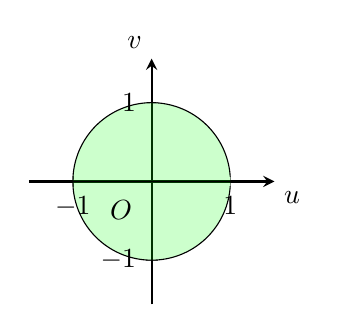
\begin{tikzpicture}
    \begin{axis}[standard,
            xtick={-1,1},
            ytick={-1,1},
            samples=1000,
            xlabel={$u$},
            ylabel={$v$},
            xmin=-1.2,xmax=1.2,
            ymin=-1.2,ymax=1.2,
            x=1cm,
            y=1cm/1
           ]
\node[anchor=center,label=south west:$O$] at (axis cs:0,0){};
\addplot[name path=F,domain={-1:1}]{sqrt(1-x^2)};
\addplot[name path=G,domain={-1:1}]{-sqrt(1-x^2)};
\addplot[name path=H,domain={-1:1}]{0};
\addplot[fill=green, fill opacity=0.2] fill between [of=F and H,soft clip={domain=-1:1}];
\addplot[fill=green, fill opacity=0.2] fill between [of=G and H,soft clip={domain=-1:1}];
    \end{axis}
    \end{tikzpicture}
}
\end{center}

Our lower and upper bounds for $u$ are $u=-1$ and $u=1$, respectively.

Our lower and upper bounds for $v$ are $v=-\sqrt{1-u^2}$ and $v=\sqrt{1-u^2}$, respectively.

Putting this all together, we get
\begin{align*}
    A&=\int_{-1}^1\int_{-\sqrt{1-u^2}}^{\sqrt{1-u^2}}ab\,dv\,du\\
    &=\int_{-1}^1\lrb{abv}_{-\sqrt{1-u^2}}^{\sqrt{1-u^2}}\,du\\
    &=\int_{-1}^1 ab\sqrt{1-u^2}-\lrp{-ab\sqrt{1-u^2}}\,du\\
    &=\int_{-1}^1 2ab\sqrt{1-u^2}\,du\\
    &=2ab\int_{-1}^1 \sqrt{1-u^2}\,du\\
    &=2ab\lrp{\frac{1}{2}\pi(1)^2}\tag{see note below}\\
    &=\boxed{ab\pi}
\end{align*}
If you love trig substitutions from 21B, you could have done $u=\sin\theta$ and do all those shenanigans. 

Unfortunately, I am lazy so I just did a shortcut. Notice that $\displaystyle \int_{-1}^1\sqrt{1-u^2}\,du$ is literally just the area of a semi-circle of radius $1$. 

This integral is similar to problem 4(c) in Homework 4 (campuswire \#18).

\phantomsection
\addcontentsline{toc}{subsection}{5(b)}\textbf{(b)} Use a similar substitution to find the volume of the ellipsoid $\displaystyle \frac{x^2}{a^2}+\frac{y^2}{b^2}+\frac{z^2}{c^2}=1$.

\Solution

Let $x=au$, $y=y=bv$, and $z=cw$. Then
\begin{align*}
    \frac{\partial x}{\partial u}=a\hspace{1em}\frac{\partial x}{\partial v}&= 0\hspace{1em}\frac{\partial x}{\partial w}=0\\
    \frac{\partial y}{\partial u}=0\hspace{1em}\frac{\partial y}{\partial v}&= b\hspace{1em}\frac{\partial y}{\partial w}=0\\
    \frac{\partial z}{\partial u}=0\hspace{1em}\frac{\partial z}{\partial v}&= 0\hspace{1em}\frac{\partial z}{\partial w}=c
\end{align*}
If you are taking / have taken linear algebra, you would immediately notice that the Jacobian for this matrix is just $abc$. Alternatively, we can take the $3\times3$ determinate using a similar process we did in 21C to find the cross product.
\begin{align*}
    \begin{vmatrix}
      \frac{\partial x}{\partial u} & \frac{\partial x}{\partial v} &
      \frac{\partial x}{\partial w}\\
      \frac{\partial y}{\partial u} & \frac{\partial y}{\partial v} &
      \frac{\partial y}{\partial w}\\
      \frac{\partial z}{\partial u} & \frac{\partial z}{\partial v} &
      \frac{\partial z}{\partial w}\\
    \end{vmatrix}&=
\begin{vmatrix}
  a & 0 & 0 \\
  0 & b & 0\\
  0 & 0 & c
\end{vmatrix}\\
&= a\begin{vmatrix}
  b & 0\\
  0 & c
\end{vmatrix}- 0\begin{vmatrix}
  0 & 0\\
  0 & c
\end{vmatrix}+0\begin{vmatrix}
  0 & b\\
  0 & 0
\end{vmatrix}\\
&= a(bc - 0) - 0(0 - 0) + 0(0 - 0)\\
&=abc
\end{align*}
Our $z$ bounds are $z=\pm c\sqrt{1- \frac{x^2}{a^2}-\frac{y^2}{b^2}}$. In terms of $u$, $v$, and $w$, our $z$ bounds are $cw=\pm c \sqrt{1- u^2 - v^2}=\implies w = \pm \sqrt{1-u^2-v^2}$.

Setting $z$ equal to $0$, we can get our $y$ bounds. Our $y$ bounds are $y=\pm b\sqrt{1-\frac{x^2}{a^2}}$. In terms of $u$, $v$, and $w$, our $y$ bounds are $bv=\pm b\sqrt{1-u^2}=\implies v=\pm \sqrt{1-u^2}$.

Setting $z$ equal to $0$ and $y$ equal to $0$, we can get our $x$ bounds. Our $x$ bounds are $x=\pm a$. In terms of $u$, $v$, and $w$, our $x$ bounds are $au=\pm a\implies u =\pm 1$.

Putting this all together, we get
\begin{align*}
    V&=\int_{-1}^1\int_{-\sqrt{1-u^2}}^{\sqrt{1-u^2}}\int_{-\sqrt{1-u^2-v^2}}^{\sqrt{1-u^2-v^2}}abc\,dw\,dv\,du\\
    &=\int_{-1}^1\int_{-\sqrt{1-u^2}}^{\sqrt{1-u^2}} 2abc\sqrt{1-u^2-v^2}\,dv\,du\\
    &=2abc\int_{0}^{2\pi}\int_{0}^1 \sqrt{1-r^2}r\,dr\,d\theta\\
    &=2abc \int_0^{2\pi}\lrb{-\frac{1}{3}(1-r^2)^{3/2}}_0^1\,d\theta\tag{convert to polar because easier}\\
    &=2abc\int_0^{2\pi} \frac{1}{3}\,d\theta\\
    &=2abc\lrb{\frac{1}{3}\theta}_0^{2\pi}\\
    &=\boxed{\frac{4\pi}{3}abc}
\end{align*}
I did this integral in a very silly way. A more efficient method would to just notice that the volume in terms of $u$, $v$, and $w$ is just a sphere with radius $1$ and then use the volume of a sphere formula. You could have also used spherical coordinates or something like that.

\phantomsection
\addcontentsline{toc}{section}{Problem 6}\textbf{Problem 6}

Show that the Jacobian for spherical coordinates $x=\rho\sin\phi\cos\theta$, $y=\rho\sin\phi\sin\theta$, $z=\rho \cos\phi$ is $\displaystyle \frac{\partial (x,y,z)}{\partial (\rho,\phi,\theta)}=\rho^2\sin\theta$.

\Solution

\phantomsection
\addcontentsline{toc}{subsection}{3x3 Determinate Method}\textbf{$3\times3$ Determinate Method}

If $x=\rho\sin\phi\cos\theta$, $y=\rho\sin\phi\sin\theta$, and $z=\rho \cos\phi$, then
\begin{align*}
    \frac{\partial x}{\partial \rho} = \sin\phi\cos\theta \hspace{1em}\frac{\partial x}{\partial \phi}& = \rho\cos\phi\cos\theta  \hspace{1em}\frac{\partial x}{\partial \theta} = -\rho \sin\phi\sin\theta\\
    \frac{\partial y}{\partial \rho} = \sin\phi\sin\theta \hspace{1em}\frac{\partial y}{\partial \phi}& = \rho\cos\phi\sin\theta  \hspace{1em}\frac{\partial y}{\partial \theta} = \rho \sin\phi\cos\theta\\
    \frac{\partial z}{\partial \rho} = \cos\phi \hspace{1em}\frac{\partial z}{\partial \phi}& = -\rho\sin\phi \hspace{2em}\frac{\partial z}{\partial \theta} =0
\end{align*}
For our Jacobian,
\begin{align*}
    \begin{vmatrix}
      \frac{\partial x}{\partial \rho} &
      \frac{\partial x}{\partial \phi} &
      \frac{\partial x}{\partial \theta}\\
      \frac{\partial y}{\partial \rho} &
      \frac{\partial y}{\partial \phi} &
      \frac{\partial y}{\partial \theta}\\
      \frac{\partial z}{\partial \rho} &
      \frac{\partial z}{\partial \phi} &
      \frac{\partial z}{\partial \theta}\\
    \end{vmatrix}&=
    \begin{vmatrix}
      \sin\phi\cos\theta & \rho\cos\phi\cos\theta & -\rho\sin\phi\sin\theta\\
      \sin\phi\sin\theta &
      \rho\cos\phi\sin\theta&
      \rho\sin\phi\cos\theta\\
      \cos\phi & -\rho\sin\phi & 0
    \end{vmatrix}\\
   &=\sin\phi\cos\theta\begin{vmatrix}
     \rho \cos\phi\sin\theta & \rho\sin\phi\cos\theta\\
     -\rho\sin\phi & 0
   \end{vmatrix}- \rho\cos\phi\cos\theta
   \begin{vmatrix}
     \sin\phi\sin\theta & \rho\sin\phi\cos\theta\\
     \cos \phi & 0
   \end{vmatrix}\\
   &\hspace{20em}-\rho\sin\phi\sin\theta
   \begin{vmatrix}
     \sin\phi\sin\theta & \rho\cos\phi\sin\theta\\
     \cos\phi &  -\rho\sin\phi
   \end{vmatrix}\\
   &=\sin\phi\cos\theta \lrp{0+\rho^2\sin^2\phi\cos\theta}-\rho\cos\phi\cos\theta\lrp{0-\rho\sin\phi\cos\phi\cos\theta}\\
   &\hspace{10em} -\rho\sin\phi\sin\theta\lrp{-\rho\sin^2\phi\sin\theta -\rho\cos^2\phi\sin\theta}\\
   &=\rho^2\sin^3\phi\cos^2\theta +\rho^2\sin\phi\cos^2\phi\cos^2\theta +\rho^2 \sin^3\phi\sin^2\theta +\rho^2\sin\phi\cos^2\phi\sin^2\theta\\
   &=\rho^2\sin^3\phi\cos^2\theta+\rho^2 \sin^3\phi\sin^2\theta+\rho^2\sin\phi\cos^2\phi\cos^2\theta+\rho^2\sin\phi\cos^2\phi\sin^2\theta\tag{rearrange terms}\\
   &=\rho^2\sin^3\phi\lrp{\cos^2\theta+\sin^2\theta}+\rho^2\sin\phi\cos^2\phi\lrp{\cos^2\theta+\sin^2\theta}\tag{factor}\\
   &=\rho^2\sin^3\phi+\rho^2\sin\phi\cos^2\phi\tag{$\cos^2 u+\sin^2u=1$}\\
   &=\rho^2\sin\phi\lrp{\sin^2\phi+\cos^2\phi}\tag{more factoring}\\
   &=\boxed{\rho^2\sin\phi}\tag{$\cos^2 u+\sin^2u=1$}
\end{align*}
If you are taking / have taken linear algebra, you would know that there is a much faster and easier way to find this $3\times3$ determinate. I am just using the method introduced in 21C.

\phantomsection
\addcontentsline{toc}{subsection}{Cylindrical Coordinates Method}\textbf{Cylindrical Coordinates Method}
\phantomsection

We know
\begin{align*}
 \frac{\partial (x,y,z)}{\partial (\rho,\phi,\theta)}=\frac{\partial (x,y,z)}{\partial (r,\theta,z)}\times \frac{\partial (r,\theta,z)}{\partial (\rho,\theta,\phi)}=\frac{\partial (x,y)}{\partial (r,\theta)}\times\frac{\partial (z, r)}{\partial(\rho,\phi)}
\end{align*}
since we can convert from Cartesian to Cylindrical to Spherical and that $z$ and $\theta$ will stay constant at certain spots.
From Cartesian to Cylindrical coordinates,
\begin{align*}
    x&=r\cos\theta\\
    y&=r\sin\theta\\
    \frac{\partial x}{\partial r} = \cos\theta &\hspace{1em}\frac{\partial x}{\partial \theta}=-r\sin\theta\\
     \frac{\partial y}{\partial r} = \sin\theta &\hspace{1em}\frac{\partial y}{\partial \theta}=r\cos\theta\\
    \begin{vmatrix}
      \frac{\partial x}{\partial r} & \frac{\partial x}{\partial \theta}\\
      \frac{\partial y}{\partial r} &
      \frac{\partial y}{\partial \theta}
    \end{vmatrix}&=\begin{vmatrix}
      \cos\theta & -r\sin\theta\\
      \sin\theta & r\cos\theta
    \end{vmatrix}=r\cos^2\theta -(r\sin^2\theta)=r(\cos^2\theta+\sin^2\theta) = r
\end{align*}
From cylindrical to spherical,
\begin{align*}
    z&=\rho\cos\phi\\
    r&=\rho\sin\phi\\
    \frac{\partial z}{\partial \rho} = \cos\phi &\hspace{1em}\frac{\partial z}{\partial \phi}=-\rho\sin\phi\\
    \frac{\partial r}{\partial \rho} = \sin\phi &\hspace{1em}\frac{\partial r}{\partial \phi}=\rho\cos\phi\\
    \begin{vmatrix}
      \frac{\partial z}{\partial \rho} & \frac{\partial z}{\partial \phi}\\
      \frac{\partial r}{\partial \rho} &
      \frac{\partial r}{\partial \phi}
    \end{vmatrix}&=\begin{vmatrix}
      \cos\phi & -\rho\sin\phi\\
        \sin\phi & \rho\cos\phi
    \end{vmatrix}=\rho\cos^2\phi -\lrp{-\rho\sin^2\phi}=\rho\lrp{\cos^2\phi+\sin^2\phi}=\rho
\end{align*}
Putting this all together (and substituting $r$ with $\rho\sin\phi$), we get
\begin{align*}
    \frac{\partial (x,y,z)}{\partial (\rho,\phi,\theta)}=r\rho=\lrp{\rho\sin\phi}\rho=\boxed{\rho^2\sin\phi}
\end{align*}
\addcontentsline{toc}{section}{Problem 7}\textbf{Problem 7}

In Math21B, you calculated the volume of the solid created by revolving the region between $y=f(x)$, $0<a<x<b$, and the $x$-axis around the $y$-axis as
\begin{align*}
    V=\int_a^b 2\pi xf(x)\,dx
\end{align*}
Verify this result using a triple integral and cylindrical coordinates.

\Solution

\textit{pls i only have ms paint}

Graphically the region looks like this in 3D


\tikzset{every picture/.style={line width=0.75pt}} %set default line width to 0.75pt        

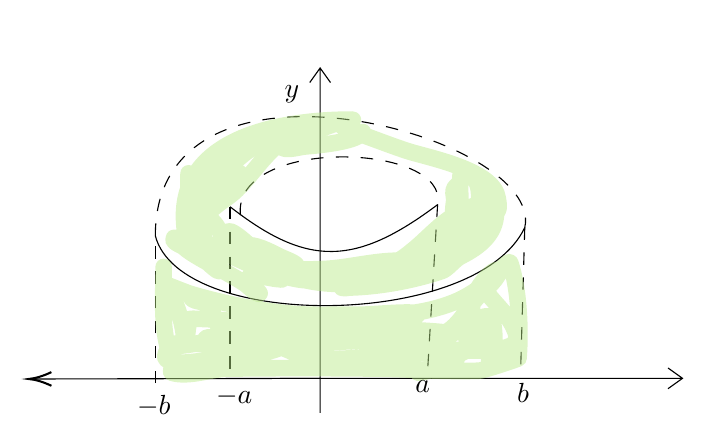
\begin{tikzpicture}[x=0.75pt,y=0.75pt,yscale=-1,xscale=1]
%uncomment if require: \path (0,300); %set diagram left start at 0, and has height of 300

%Shape: Axis 2D [id:dp43042752003169704] 
\draw  (181,214.51) -- (375,214.51)(200.4,65) -- (200.4,231.12) (368,209.51) -- (375,214.51) -- (368,219.51) (195.4,72) -- (200.4,65) -- (205.4,72)  ;
%Straight Lines [id:da38160510227408195] 
\draw    (200.4,214.51) -- (62,214.83) ;
\draw [shift={(60,214.83)}, rotate = 359.87] [color={rgb, 255:red, 0; green, 0; blue, 0 }  ][line width=0.75]    (10.93,-3.29) .. controls (6.95,-1.4) and (3.31,-0.3) .. (0,0) .. controls (3.31,0.3) and (6.95,1.4) .. (10.93,3.29)   ;
%Curve Lines [id:da06413463988732948] 
\draw    (157,131.83) .. controls (194,160.67) and (217,160.83) .. (257,130.83) ;
%Curve Lines [id:da20988816584554137] 
\draw    (121,145.83) .. controls (133,191.83) and (276,190.83) .. (299,141.83) ;
%Straight Lines [id:da6724536987718275] 
\draw  [dash pattern={on 4.5pt off 4.5pt}]  (121,216.83) -- (121,145.83) ;
%Straight Lines [id:da23554100812811996] 
\draw  [dash pattern={on 4.5pt off 4.5pt}]  (157,131.83) -- (157,211.83) ;
%Straight Lines [id:da14143823650582066] 
\draw  [dash pattern={on 4.5pt off 4.5pt}]  (257,130.83) -- (252,213.83) ;
%Straight Lines [id:da36511803145286104] 
\draw  [dash pattern={on 4.5pt off 4.5pt}]  (299,141.83) -- (297,210.83) ;
%Curve Lines [id:da7955483070135249] 
\draw  [dash pattern={on 4.5pt off 4.5pt}]  (162,135.83) .. controls (158,97.83) and (263,100.83) .. (257,130.83) ;
%Curve Lines [id:da07731462746671558] 
\draw  [dash pattern={on 4.5pt off 4.5pt}]  (121,145.83) .. controls (121,45.83) and (309,97.83) .. (299,141.83) ;
%Shape: Free Drawing [id:dp6671211115273981] 
\draw  [color={rgb, 255:red, 184; green, 233; blue, 134 }  ,draw opacity=0.46 ][line width=6] [line join = round][line cap = round] (277,134.83) .. controls (272.71,151.98) and (261.38,156.37) .. (245,161.83) .. controls (244.15,162.12) and (252.87,154.34) .. (254,152.83) .. controls (259.87,145.01) and (268.32,139.52) .. (275,132.83) .. controls (275.67,132.17) and (273.52,134.05) .. (273,134.83) .. controls (270.84,138.07) and (268.86,141.42) .. (267,144.83) .. controls (262.66,152.8) and (251.53,155.41) .. (243,156.83) .. controls (241.23,157.13) and (239.27,160.1) .. (238,158.83) .. controls (237.76,158.6) and (237.7,157.98) .. (238,157.83) .. controls (240.56,156.55) and (242.76,154.62) .. (245,152.83) .. controls (252.57,146.78) and (258.99,138.55) .. (269,133.83) .. controls (273.86,131.54) and (284.33,126.5) .. (285,131.83) .. controls (286.55,144.25) and (277.41,151.13) .. (268,155.83) .. controls (265.26,157.2) and (261.75,161.92) .. (259,162.83) .. controls (244.27,167.74) and (226.92,170.83) .. (211,170.83) .. controls (210,170.83) and (213.09,171.24) .. (214,170.83) .. controls (216.2,169.86) and (217.91,168.03) .. (220,166.83) .. controls (223.18,165.02) and (229.52,162.07) .. (232,160.83) .. controls (234,159.83) and (240.24,157.83) .. (238,157.83) .. controls (226.05,157.83) and (213.27,161.4) .. (202,161.83) .. controls (193.67,162.15) and (185.33,162.15) .. (177,161.83) .. controls (176.52,161.82) and (174,159.83) .. (174,159.83) .. controls (174,159.83) and (175.28,160.65) .. (176,160.83) .. controls (182.55,162.47) and (188.88,161.77) .. (195,164.83) .. controls (196.61,165.64) and (201.7,166.27) .. (200,166.83) .. controls (192.91,169.2) and (184.67,159.83) .. (178,159.83) .. controls (176.8,159.83) and (179.93,161.3) .. (181,161.83) .. controls (183.27,162.97) and (185.54,164.22) .. (188,164.83) .. controls (193.67,166.25) and (210.14,165.83) .. (212,165.83) .. controls (213.05,165.83) and (210.04,166.68) .. (209,166.83) .. controls (207.02,167.12) and (204.98,166.55) .. (203,166.83) .. controls (196.13,167.81) and (191.34,167.42) .. (185,165.83) .. controls (173.64,162.99) and (162.55,158.11) .. (152,152.83) .. controls (151.83,152.75) and (141.07,146.3) .. (140,146.83) .. controls (138.87,147.4) and (142.45,150.7) .. (143,150.83) .. controls (149.3,152.41) and (162.41,155.72) .. (169,153.83) .. controls (169.99,153.55) and (157.84,141.99) .. (156,143.83) .. controls (154.3,145.53) and (163.34,149.31) .. (164,149.83) .. controls (168.2,153.19) and (173.14,155.54) .. (178,157.83) .. controls (180.2,158.87) and (182.75,158.93) .. (185,159.83) .. controls (186.38,160.39) and (187.95,162.89) .. (189,161.83) .. controls (191.36,159.48) and (183.98,157.32) .. (181,155.83) .. controls (177.32,153.99) and (168,148.84) .. (164,150.83) .. controls (162.18,151.74) and (173.94,161.79) .. (174,161.83) .. controls (176.22,163.65) and (178.57,165.31) .. (181,166.83) .. controls (181.28,167.01) and (182.33,166.83) .. (182,166.83) .. controls (176.66,166.83) and (171.07,164.14) .. (166,165.83) .. controls (165.55,165.98) and (166.67,166.5) .. (167,166.83) .. controls (168.24,168.07) and (168.3,169.44) .. (169,170.83) .. controls (169.54,171.91) and (172.2,173.83) .. (171,173.83) .. controls (169.41,173.83) and (165.68,169.95) .. (164,168.83) .. controls (156.24,163.66) and (145.37,158.74) .. (138,153.83) .. controls (132.92,150.45) and (133.68,149.52) .. (131,146.83) .. controls (130.76,146.6) and (130.24,146.6) .. (130,146.83) .. controls (128.4,148.43) and (132.94,150.3) .. (134,150.83) .. controls (137.07,152.37) and (140.14,153.93) .. (143,155.83) .. controls (144.27,156.68) and (151.07,163.76) .. (152,162.83) .. controls (152.85,161.98) and (150.54,160.91) .. (150,159.83) .. controls (148.53,156.9) and (147.32,153.84) .. (146,150.83) .. controls (140.32,137.86) and (140.5,125.5) .. (148,113.83) .. controls (151.59,108.25) and (159.42,105.88) .. (165,102.83) .. controls (176.2,96.72) and (193.66,88.78) .. (207,90.83) .. controls (209.52,91.22) and (211.77,94.09) .. (214,94.83) .. controls (223.46,97.99) and (232.36,101.62) .. (242,104.83) .. controls (251.74,108.08) and (284.26,113.93) .. (286,127.83) .. controls (286.25,129.82) and (286.89,132.04) .. (286,133.83) .. controls (285.55,134.73) and (283.83,133.28) .. (283,133.83) .. controls (281.61,134.76) and (280.86,136.4) .. (280,137.83) .. controls (279.27,139.05) and (277.08,142.25) .. (277,140.83) .. controls (276.22,126.85) and (279.86,119.76) .. (270,114.83) .. controls (269.27,114.47) and (268.03,116.29) .. (268,116.83) .. controls (267.69,122.16) and (268,127.5) .. (268,132.83) .. controls (268,133.92) and (268.12,120.77) .. (266,121.83) .. controls (263.54,123.06) and (265.21,127.38) .. (265,128.83) .. controls (263.96,136.1) and (264.35,143.5) .. (264,150.83) .. controls (263.93,152.35) and (253.76,155.59) .. (253,155.83) .. controls (244.67,158.5) and (236.12,160.58) .. (228,163.83) .. controls (223.12,165.79) and (218.23,168.4) .. (213,168.83) .. controls (192.82,170.52) and (159.76,159.35) .. (151,141.83) .. controls (149.55,138.93) and (145.02,135.9) .. (144,132.83) .. controls (142.77,129.15) and (146.32,126.35) .. (148,123.83) .. controls (154.58,113.96) and (160.64,108.07) .. (170,101.83) .. controls (172.58,100.11) and (178.3,97.45) .. (182,96.83) .. controls (183.32,96.61) and (184.69,97.09) .. (186,96.83) .. controls (186.73,96.69) and (188.41,95.21) .. (188,95.83) .. controls (185.86,99.04) and (180.29,101.71) .. (178,103.83) .. controls (171.17,110.18) and (165.84,118.52) .. (159,124.83) .. controls (156.55,127.09) and (153.6,128.75) .. (151,130.83) .. controls (150.38,131.33) and (146.16,135) .. (146,134.83) .. controls (145.67,134.5) and (146.65,134.15) .. (147,133.83) .. controls (150.49,130.66) and (153.96,127.43) .. (157,123.83) .. controls (158.93,121.56) and (163.67,114.5) .. (161,115.83) .. controls (155.32,118.68) and (148.68,125.78) .. (145,129.83) .. controls (144.78,130.08) and (145.15,130.54) .. (145,130.83) .. controls (143.84,133.16) and (138.2,156.27) .. (137,141.83) .. controls (136.7,138.18) and (137,134.5) .. (137,130.83) .. controls (137,82.85) and (137.31,166.23) .. (135,140.83) .. controls (131.04,97.25) and (183.95,89.83) .. (216,89.83) .. controls (217.7,89.83) and (212.65,90.42) .. (211,90.83) .. controls (207.93,91.6) and (205,92.83) .. (202,93.83) .. controls (197.38,95.37) and (178.97,93.71) .. (181,101.83) .. controls (181.97,105.73) and (189.01,103.29) .. (193,102.83) .. controls (196.08,102.48) and (218.4,101.04) .. (221,95.83) ;
%Shape: Free Drawing [id:dp4635645905492446] 
\draw  [color={rgb, 255:red, 184; green, 233; blue, 134 }  ,draw opacity=0.46 ][line width=6] [line join = round][line cap = round] (125,160.83) .. controls (125,170.31) and (124.09,184.33) .. (126,194.83) .. controls (126.85,199.53) and (128.1,204.33) .. (129,208.83) .. controls (129.2,209.81) and (128.04,211.55) .. (129,211.83) .. controls (137.1,214.26) and (147.77,209.94) .. (156,209.83) .. controls (180,209.52) and (204,209.51) .. (228,209.83) .. controls (244.34,210.05) and (260.68,211.46) .. (277,210.83) .. controls (278.94,210.76) and (295.97,205.18) .. (296,204.83) .. controls (297.07,190.94) and (296.23,171.53) .. (292,158.83) .. controls (291.33,156.83) and (284.4,165.81) .. (283,166.83) .. controls (277.33,170.99) and (271.53,175.22) .. (265,177.83) .. controls (243.37,186.49) and (219.18,184.29) .. (195,183.83) .. controls (178.03,183.51) and (154.25,178.71) .. (138,173.83) .. controls (136.04,173.25) and (125,168.83) .. (125,168.83) .. controls (125,168.83) and (128.89,174.62) .. (129,174.83) .. controls (132.45,181.72) and (135,190.39) .. (135,197.83) .. controls (135,198.58) and (135.82,196.56) .. (136,195.83) .. controls (136.29,194.68) and (136.88,185.84) .. (138,185.83) .. controls (174,185.49) and (213.8,200.93) .. (246,184.83) .. controls (253.46,181.1) and (229.34,183.6) .. (221,183.83) .. controls (212.38,184.07) and (195.22,182.72) .. (187,186.83) .. controls (186.58,187.04) and (187.53,187.79) .. (188,187.83) .. controls (191.32,188.14) and (194.67,187.67) .. (198,187.83) .. controls (209.14,188.36) and (219.87,191.33) .. (231,191.83) .. controls (235,192.01) and (247,191.83) .. (243,191.83) .. controls (225,191.83) and (171,191.83) .. (189,191.83) .. controls (206.04,191.83) and (241.54,189.62) .. (264,192.83) .. controls (264.74,192.94) and (262.73,193.7) .. (262,193.83) .. controls (259.03,194.37) and (256.01,194.68) .. (253,194.83) .. controls (229.01,196.02) and (205.01,197.25) .. (181,197.83) .. controls (164.01,198.25) and (147,197.83) .. (130,197.83) .. controls (126,197.83) and (138.01,198.07) .. (142,197.83) .. controls (148.81,197.43) and (158.06,198.8) .. (164,195.83) .. controls (165.66,195) and (157.28,191.55) .. (160,188.83) .. controls (169.46,179.37) and (190.04,189.36) .. (201,191.83) .. controls (207.25,193.25) and (213.6,194.45) .. (220,194.83) .. controls (230.31,195.45) and (240.67,195.13) .. (251,194.83) .. controls (264.14,194.46) and (267.42,186.31) .. (275,176.83) .. controls (278.68,172.23) and (284.81,168.68) .. (287,162.83) .. controls (287.35,161.9) and (284.83,162.28) .. (284,162.83) .. controls (281.65,164.4) and (279.64,166.53) .. (278,168.83) .. controls (276.27,171.26) and (274.68,173.93) .. (274,176.83) .. controls (273.31,179.75) and (273.67,182.85) .. (274,185.83) .. controls (274.19,187.58) and (283.07,186.13) .. (281,185.83) .. controls (274.02,184.84) and (269.09,188.2) .. (271,195.83) .. controls (271.52,197.9) and (274.05,192.74) .. (275,190.83) .. controls (276.56,187.72) and (277.31,183.66) .. (282,184.83) .. controls (284.82,185.54) and (284.62,199.58) .. (284,204.83) .. controls (283.86,206.03) and (282.14,209.03) .. (282,207.83) .. controls (281.3,201.87) and (283.46,184.01) .. (282,189.83) .. controls (279.74,198.89) and (259.94,206.36) .. (255,208.83) .. controls (252.73,209.97) and (245.46,211.83) .. (248,211.83) .. controls (248.73,211.83) and (266,208.12) .. (266,205.83) .. controls (266,202.54) and (252.64,200.95) .. (249,199.83) .. controls (245.67,198.81) and (242.11,198.39) .. (239,196.83) .. controls (238.7,196.68) and (238.67,195.86) .. (239,195.83) .. controls (247.47,195.23) and (258.35,197.57) .. (266,191.83) .. controls (273.1,186.51) and (271.74,173.67) .. (279,168.83) .. controls (279.83,168.28) and (281.71,174.48) .. (282,174.83) .. controls (286.9,180.71) and (293.13,186.37) .. (295,193.83) .. controls (297.43,203.56) and (267.67,200.72) .. (265,200.83) .. controls (262.31,200.95) and (259.69,201.74) .. (257,201.83) .. controls (245.3,202.25) and (207.56,206.5) .. (197,204.83) .. controls (186.58,203.19) and (176.18,195.3) .. (166,194.83) .. controls (159.34,194.53) and (152.66,194.52) .. (146,194.83) .. controls (145.26,194.87) and (144.25,196.81) .. (145,196.83) .. controls (157,197.17) and (169,196.83) .. (181,196.83) .. controls (182.05,196.83) and (179.05,195.88) .. (178,195.83) .. controls (170.67,195.53) and (163.32,195.35) .. (156,195.83) .. controls (148.29,196.35) and (140.68,197.95) .. (133,198.83) .. controls (130.37,199.14) and (128.95,197.91) .. (127,200.83) .. controls (118.31,213.87) and (158.33,202.16) .. (174,201.83) .. controls (175.48,201.8) and (179.66,200.5) .. (181,199.83) .. controls (181.94,199.36) and (185.05,198.83) .. (184,198.83) .. controls (174.07,198.83) and (162.26,199.72) .. (154,192.83) .. controls (149.69,189.24) and (149.74,182.58) .. (146,178.83) .. controls (144.39,177.22) and (138,177.81) .. (138,174.83) ;

% Text Node
\draw (182,72.4) node [anchor=north west][inner sep=0.75pt]    {$y$};
% Text Node
\draw (245,214.4) node [anchor=north west][inner sep=0.75pt]    {$a$};
% Text Node
\draw (294,215.4) node [anchor=north west][inner sep=0.75pt]    {$b$};
% Text Node
\draw (149,217.4) node [anchor=north west][inner sep=0.75pt]    {$-a$};
% Text Node
\draw (111,221.4) node [anchor=north west][inner sep=0.75pt]    {$-b$};


\end{tikzpicture}


Our front view looks like
\begin{center}
\resizebox{3.5cm}{!}{
    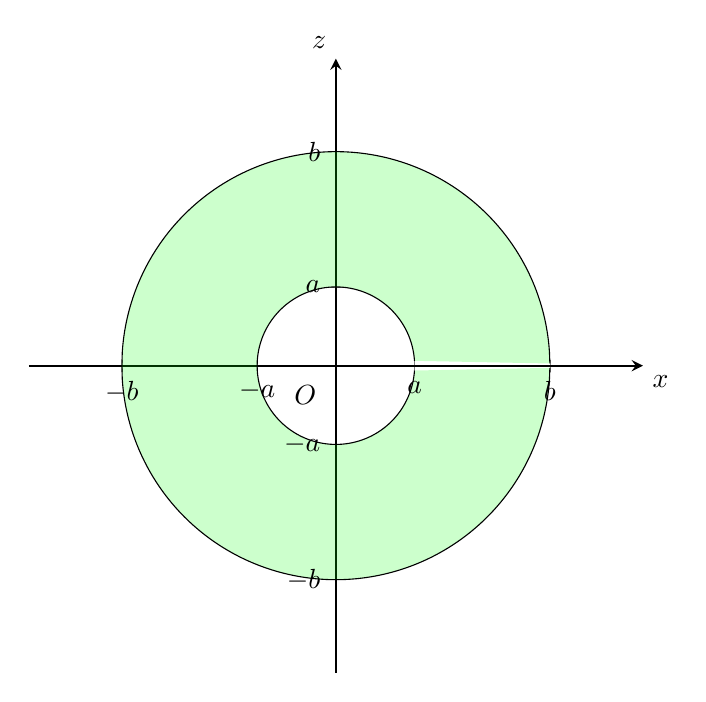
\begin{tikzpicture}
    \begin{axis}[standard,
            xtick={-2.718,-1,1,2.718},
            ytick={-2.718,-1,1,2.718},
            samples=1000,
            xlabel={$x$},
            ylabel={$z$},
            xmin=-3,xmax=3,
            ymin=-3,ymax=3,
            x=1cm,
            y=1cm/1,
            xticklabels={$-b$, $-a$, $a$, $b$},
            yticklabels={$-b$, $-a$, $a$, $b$}
           ]
\node[anchor=center,label=south west:$O$] at (axis cs:0,0){};
\addplot[name path=F,domain={-2.718:2.718}]{sqrt(2.718^2-x^2};
\addplot[name path=G,domain={-2.718:2.718}]{-sqrt(2.718^2-x^2};
\addplot[name path=H,domain={-1:1}]{sqrt(1-x^2)};
\addplot[name path=I,domain={-1:1}]{-sqrt(1-x^2)};
\addplot[fill=green, fill opacity=0.2] fill between [of=F and H, soft clip={domain=-2.718:2.718}];
\addplot[fill=green, fill opacity=0.2] fill between [of=G and I, soft clip={domain=-2.718:2.718}];
    \end{axis}
    \end{tikzpicture}
}
\end{center}
Our lower and upper bounds for $r$ will be $r=a$ and $r=b$, respectively. 

Our lower and upper bounds for $\theta$ will be $\theta=0$ and $\theta=2\pi$, respectively.

Our upper and lower bounds for $y$ will just be $y=0$ and $y=f(r)$, respectively. The reason why it's $f(r)$ is that every ``radius" corresponds with a certain height ($y$ value).

The order of for this volume integral does not particularly matter, but trust me when I saw that we want to have $r$ on the outside.
\begin{align*}
    V&=\int_a^b\int_0^{2\pi}\int_0^{f(r)}r\,dy\,d\theta\,dr\\
    &=\int_a^b\int_0^{2\pi}\lrb{ry}_0^{f(r)}\,d\theta\,dr\\
    &=\int_a^b\int_0^{2\pi} rf(r)\,d\theta\,dr\\
    &=\int_a^b\lrb{rf(r)\theta}_0^{2\pi}\,dr\\
    &=\int_a^b 2\pi rf(r)\,dr\\
    &=\boxed{\int_a^b 2\pi xf(x)\,dr}
\end{align*}
We were able to do that last step because $r$ is pretty much a placeholder variable. We can just replace the letter $r$ with the letter $x$ to get the exact answer we want.
\end{document}
